\documentclass[12pt]{article}
\usepackage[utf8]{inputenc} % For UTF-8 support
\usepackage[T1]{fontenc}    % For better font encoding
\usepackage{textcomp}       % For special characters
\usepackage{amsmath, amssymb}
\usepackage{graphicx}
\usepackage{amsthm} 
\usepackage{hyperref}
\usepackage{float}
\usepackage{listings}
\usepackage{xcolor}
\usepackage{multirow}
\usepackage{subcaption}
\usepackage{booktabs}


% Define keywords environment manually
\providecommand{\keywords}[1]{\textbf{Keywords:} #1}


% Define the 'remark' environment
\newtheoremstyle{remarkstyle} % Define a custom style
{5pt}      % Space above
{5pt}      % Space below
{}         % Body font
{}         % Indentation
{\bfseries} % Header font
{.}        % Punctuation after header
{ }        % Space after header
{\thmname{#1}\thmnumber{ #2}\thmnote{ (#3)}} % Header format

\theoremstyle{remarkstyle}
\newtheorem{remark}{Remark}
\usepackage{tikz}
\usepackage[english]{babel}
\usepackage[numbers]{natbib} % Enables numeric citation style with natbib package
\bibliographystyle{unsrtnat} % Sets the bibliography style to unsrtnat, which lists references in the order they are cited
\usetikzlibrary{positioning}

% Page margins
\usepackage[a4paper, margin=1in]{geometry}
\newtheorem{definition}{Definition}
\newtheorem{theorem}{Theorem} 
% Line spacing
\usepackage{algorithm}
\usepackage{graphicx}
\usepackage{caption}
\usepackage{multicol}
\usepackage{algpseudocode}
\usepackage{setspace}
\onehalfspacing

% Custom headers and footers
\usepackage{fancyhdr}
\pagestyle{fancy}
\fancyhf{}
\rhead{MATH3999 Directed Studies}
\lhead{LIU Zhonglin}
\rfoot{Page \thepage}

\title{
	{Various Travelling Salesman Problems}\\
	
	{
\includegraphics[width=8cm]{Figures/logo}} 
}
\author{
	Liu Zhonglin \\[1em] % Your name, followed by a 1em vertical space
	\normalsize{MATH3999: Directed Studies in Mathematics} \\[1em] % Course info, followed by a larger 2em vertical space
	\normalsize{Supervised by: Prof. Zang Wenan} % Supervisor info
}
\date{2024-2025 Semester 1}


\begin{document}
	
	\maketitle
	
\begin{abstract}
	This study investigates both classical and modern approaches to the Traveling Salesman Problem (TSP), comparing traditional approximation algorithms with deep reinforcement learning methods. We implement and analyze two classical heuristics---the Quick Insertion Method (2-approximation) and Christofides algorithm (1.5-approximation)---alongside three reinforcement learning agents based on Pointer Networks with attention mechanisms. The RL approaches include pure REINFORCE training, hybrid REINFORCE with Christofides initialization, and hybrid Actor-Critic methods. Through comprehensive evaluation on randomly generated instances for both 30-city and 100-city problems, we demonstrate that classical heuristics consistently outperform pure RL agents in both solution quality and computational efficiency. However, hybrid approaches that leverage classical algorithms for input ordering show dramatic improvements, with the Actor-Critic hybrid model achieving performance statistically equivalent to classical methods on larger instances. These findings suggest that the promising direction for machine learning in combinatorial optimization lies not in replacing classical methods, but in creating intelligent hybrid systems that combine the structural insights of traditional algorithms with the adaptive capabilities of modern neural networks.
\end{abstract}

\keywords{Traveling Salesman Problem, reinforcement learning, pointer networks, approximation algorithms, hybrid methods}
	

	\newpage
	
\section{Introduction}

The Traveling Salesman Problem (TSP) stands as one of the most studied problems in combinatorial optimization, serving as a cornerstone for understanding computational complexity and algorithmic design \cite{applegate2011traveling}. Given a set of cities and distances between them, the TSP seeks the shortest possible route that visits each city exactly once and returns to the starting point. Despite its simple formulation, the TSP is NP-hard, making exact solutions computationally intractable for large instances \cite{hartmanis1982computers}.

Classical approaches to the TSP have predominantly focused on approximation algorithms that provide polynomial-time solutions with theoretical performance guarantees. Notable among these are the Quick Insertion Method, which achieves a 2-approximation ratio, and the celebrated Christofides algorithm \cite{christofides2022worst}, which provides a 1.5-approximation for metric TSP instances. These algorithms have remained the gold standard for decades due to their efficiency and reliability.

Recent advances in deep learning have sparked renewed interest in applying neural networks to combinatorial optimization problems. Pointer Networks \cite{vinyals2015pointer} have emerged as a particularly promising architecture for sequence-to-sequence problems where the output is a permutation of the input. Subsequent work has explored reinforcement learning approaches, with policy gradient methods like REINFORCE \cite{williams1992simple} and Actor-Critic algorithms \cite{sutton1998reinforcement} showing potential for learning effective TSP heuristics.

However, the relative performance of these modern learning-based methods compared to classical algorithms remains an open question, particularly regarding their scalability and practical applicability. Furthermore, the potential for hybrid approaches that combine the strengths of both paradigms has received limited systematic investigation.

This study provides a comprehensive comparison of classical approximation algorithms and deep reinforcement learning methods for the TSP. We implement both traditional heuristics and state-of-the-art neural approaches, evaluating their performance across different problem scales. Our key contribution lies in demonstrating that hybrid methods, which leverage classical algorithms to guide neural network training, can achieve performance competitive with established heuristics while maintaining the adaptive capabilities of learning-based systems.


	
	
	
	\section{Preliminaries and Problem Formulation}
	Before delving into the problem formulation of the TSP, it is essential to introduce several foundational concepts that play a critical role in understanding and solving the problem.\\
	Let \( G = (V, E) \) be a graph where \( V \) is the set of vertices and \( E \) is the set of edges.
	
	\begin{definition}[Matching]
		In a graph \( G = (V, E) \), a \textit{matching} is a subset of edges \( M \subseteq E \) such that no two edges share a common vertex. A matching $M$ is called perfect matching if $\displaystyle \lvert M\rvert=\frac{\lvert V\rvert}{2},$ i.e. each vertex of $G$ is incident with an edge in M.
	\end{definition}
	
	\begin{theorem}
		Let $G$ be a graph with a weight $w(e)$ on each edge. Then the maximum-weight matching, maximum-weight perfect matching, minimum-weight matching, and minimum-weight perfect matching problems can be solved in polynomial time. 
	\end{theorem}
	
	\begin{definition}[Minimum Spanning Tree]
		In a connected, edge-weighted graph \( G = (V, E) \), a \textit{Minimum Spanning Tree (MST)} is a subset of the edges \( T \subseteq E \) that connects all the vertices together without any cycles and with the minimum possible total edge weight. 
	\end{definition}
	
	\begin{definition}[Hamiltonian Cycle]
		In a graph \( G = (V, E) \), a \textit{Hamiltonian cycle} is a cycle that visits each vertex exactly once and returns to the starting vertex. 
	\end{definition}
	
	
	\begin{definition}[Eulerian Tour]
		In a graph \( G = (V, E) \), an \textit{Eulerian tour} is a tour that visits every edge exactly once and returns to the starting vertex.
	\end{definition}
	
	\begin{definition}[Eulerian Graph]
		A graph \( G = (V, E) \) is called an \textit{Eulerian graph} if there exists an Eulerian tour in the graph. 
	\end{definition}
	
	\begin{theorem}[Characterization of Eulerian Graphs]
		A connected graph \( G = (V, E) \) is Eulerian if and only if every vertex of the graph has an even degree.
	\end{theorem}
	
We will now introduce classical algorithms for finding spanning trees and Eulerian tours in Eulerian graphs.\\
	Kruskal's algorithm and Prim's algorithm process a connected graph \( G = (V, E) \) with a weight \( w(e) \) on each edge \( e \), and output the minimum spanning tree of the graph.
	
	\begin{algorithm}[htb]
		\caption{Kruskal's Algorithm}
		\begin{algorithmic}[1]
			\State \( F \gets \emptyset \)
			\For{\( v \in V \)}
			\State \textsc{Make-Set}(\( v \))
			\EndFor
			\State Sort all edges \( e \in E \) by weight \( w(e) \), in non-decreasing order
			\For{\textbf{each} edge \( \{u, v\} \) in the sorted list}
			\If{\textsc{Find-Set}(\( u \)) \(\neq\) \textsc{Find-Set}(\( v \))}
			\State \( F \gets F \cup \{ \{u, v\} \} \)
			\State \textsc{Union}(\textsc{Find-Set}(\( u \)), \textsc{Find-Set}(\( v \)))
			\EndIf
			\EndFor
			\State \Return \( F \)
		\end{algorithmic}
	\end{algorithm}
	
	\begin{algorithm}[H]
		\caption{Prim's Algorithm}
		\begin{algorithmic}[1]
			\State Find the edge \( e = \{u, v\} \) in \( E \) with the minimum weight \( w(e) \)
			\State Initialize the tree \( T \) with the edge \( e \), \( T := \{e\} \)
			\State Initialize the set of vertices in \( T \), \( V_T := \{u, v\} \)
			\While{\( |V_T| < |V| \)}
			\State Find the edge \( \{x, y\} \) in \( E \) with the minimum weight \( w(\{x, y\}) \), where \( x \in V_T \) and \( y \notin V_T \)
			\State Add \( \{x, y\} \) to \( T \)
			\State Add \( y \) to \( V_T \)
			\EndWhile
			\State \textbf{return} \( T \)
		\end{algorithmic}
	\end{algorithm}
	
	Fleury's algorithm is designed to find an Eulerian tour in a graph.
	
	\begin{algorithm}
		\caption{Fleury’s Algorithm}
		\begin{algorithmic}[1]
			\State Choose an arbitrary vertex \( v_0 \).
			\State Initialize \( tour = [v_0] \).
			\While{there are unused edges in the graph}
			\State Let \( v \) be the current vertex at the end of the last added edge in \( tour \) (start with \( v_0 \)).
			\State Choose \( e \) from the edges connected to \( v \) such that $e$ is not a bridge, unless no other option exists.
			\State Add \( e \) and the vertex at the other end of \( e \) to \( tour \).
			\State Remove \( e \) from the graph.
			\EndWhile
			\State \textbf{return} \( tour \)
		\end{algorithmic}
	\end{algorithm}

	
	
	
	
	

	\textbf{Travelling salesman problem}:\\
	A salesman wishes to make a tour, visiting each of $n$ cities exactly once and finishing at tyhe city he starts from. Suppose there is a road between any two cities and the road between city $i$ and city $j$ is of distance $w_{ij}$. The objective of the salesman is to find such a tour with the minimum total distance.\\
	This problem can be formulated in the following form:\\
	
	\noindent \textbf{Travelling salesman problem}(Equivalent Form):\\
	\textbf{Input}: A complete graph $G=(V,E)$ with a weight $w_{ij}$ on each edge $ij.$\\
	\textbf{Output}: A Hamiltonian cycle of $G$ with minimum total weight.
	
	\section{Classical Approximation Algorithms}
	Since the TSP is $NP$-hard, there is no polynomial-time algorithm for solving it unless $NP=P$. So scientists turn to search for approximation algorithm.\\
	A polynomial-time algorithm is said to be a \textbf{$\delta$-approximation algorithm} for TSP if for every instance $I$, it delivers a Hamiltonian cycle $C$ such that 
	$$\frac{w(C)}{w(C^\star)}\leq \delta,$$ 
	where $C^\star$ is a Hamiltonian cycle of $I$ with minimum total weight.\\
	A weight function $w$ defined on a complete graph $G$ is said to satisfy the \textbf{triangle-inequality} if for any three vertices $i,j,k$ of $G$, $$w_{ij}+w_{jk}\geq w_{ik}.$$ In this project we shall investigate some approximation algorithms for the TSP satisfying triangle-inequalities. Let $G=(V,E)$ be a complete graph with a nonnegative integral weight on each edge, and the weight function satisfies triangle-inequality.
	
	\subsection{Quick Insertion Method}
	\begin{algorithm}
		\caption{Quick Insertion Method}
		\begin{algorithmic}[1] % The number [1] indicates that lines are numbered
			\State Compute a minimum spanning tree $T$ in $G$.
			\State Let $H$ be the multigraph obtained from $T$ be duplicating each edge once. Compute an Eulerian tour $W$ of $H$, and connect $W$ into a Hamiltanian cycle $C$ by making a shortcut. Return $C$.
			
		\end{algorithmic}
	\end{algorithm}
	
	

	
\begin{multicols}{2}
	% Left Graph (labeled as T)
	\begin{tikzpicture}[node distance=1cm and 1cm, every node/.style={draw, circle, inner sep=2pt}]
		% Add Label for the Graph
		\node[draw=none] at (0, 2) {\textbf{$T$}};
		
		% Nodes
		\node (1) {1};
		\node (2) [below=of 1] {2};
		\node (3) [below left=of 2] {3};
		\node (4) [below right=of 2] {4};
		\node (5) [above right=of 1] {5};
		\node (6) [below right=of 5] {6};
		\node (7) [below left=of 6] {7};
		\node (8) [below right=of 6] {8};
		
		% Edges
		\draw (1) -- (2);
		\draw (2) -- (3);
		\draw (2) -- (4);
		\draw (1) -- (5);
		\draw (5) -- (6);
		\draw (6) -- (7);
		\draw (6) -- (8);
	\end{tikzpicture}
	
	\columnbreak
	
	% Right Graph (labeled as H)
	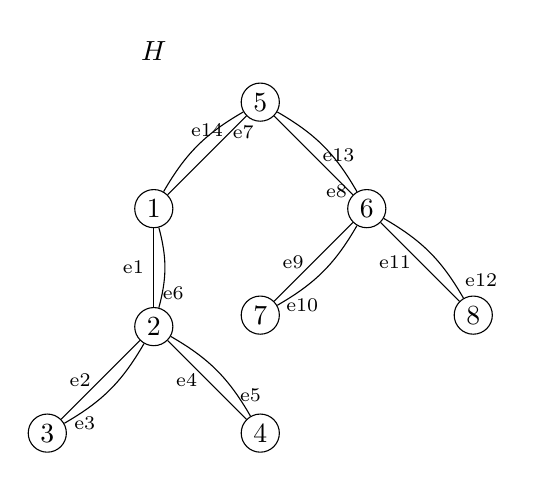
\begin{tikzpicture}[node distance=1cm and 1cm, every node/.style={draw, circle, inner sep=2pt}]
		% Add Label for the Graph
		\node[draw=none] at (0, 2) {\textbf{$H$}};
		
		% Nodes
		\node (1') {1};
		\node (2') [below=of 1'] {2};
		\node (3') [below left=of 2'] {3};
		\node (4') [below right=of 2'] {4};
		\node (5') [above right=of 1'] {5};
		\node (6') [below right=of 5'] {6};
		\node (7') [below left=of 6'] {7};
		\node (8') [below right=of 6'] {8};
		
		% Edges with Labels
		\draw (1') -- (2') node[midway, left, draw=none] {\scriptsize e1};
		\draw (1') to[bend left=15] (2') node[above right, draw=none] {\scriptsize e6};
		\draw (2') -- (3') node[midway, left, draw=none] {\scriptsize e2};
		\draw (2') to[bend left=15] (3') node[right, draw=none] {\scriptsize e3};
		\draw (2') -- (4') node[midway, left, draw=none] {\scriptsize e4};
		\draw (2') to[bend left=15] (4') node[above, draw=none] {\scriptsize e5};
		\draw (1') -- (5') node[midway, above, draw=none] {\scriptsize e14};
		\draw (1') to[bend left=15] (5') node[below, draw=none] {\scriptsize e7};
		\draw (5') -- (6') node[midway, right, draw=none] {\scriptsize e13};
		\draw (5') to[bend left=15] (6') node[left, draw=none] {\scriptsize e8};
		\draw (6') -- (7') node[midway, left, draw=none] {\scriptsize e9};
		\draw (6') to[bend left=15] (7') node[right, draw=none] {\scriptsize e10};
		\draw (6') -- (8') node[midway, left, draw=none] {\scriptsize e11};
		\draw (6') to[bend left=15] (8') node[above right, draw=none] {\scriptsize e12};
	\end{tikzpicture}
\end{multicols}

\begin{remark}
	Recall that $W$ is a sequence where terms are alternately vertices and edges. The short cut can be produced by listing the vertices when they're first encountered in $W$. Suppose $T$ is as depicted above. Then an Eulerian tour on $H$ is 
	$$W=1e_12e_23e_32e_44e_52e_61e_75e_86e_97e_{10}6e_{11}8e_{12}6e_{13}5e_{14}1.$$
	Then $C=123456781$ is the desired Hamiltonian cycle. Since the weight function satisfies triangle inequality, $w_{34}\leq w(e_3)+w(e_4),w_{45}\leq w(e_5)+w(e_6)+w(e_7), w_{78}\leq w(e_{10})+w(e_{11}),w_{81}\leq w(e_{12})+w(e_{13})+w(e_{14}).$ Thus $w(C)\leq w(W)\leq 2w(C^\star).$
	
	
	
\end{remark}
	
Below is a graph illustrating the implementation of the algorithm. The resulting tour is $[0, 1, 6, 2, 3, 4, 5, 0].$ 
\begin{center}
	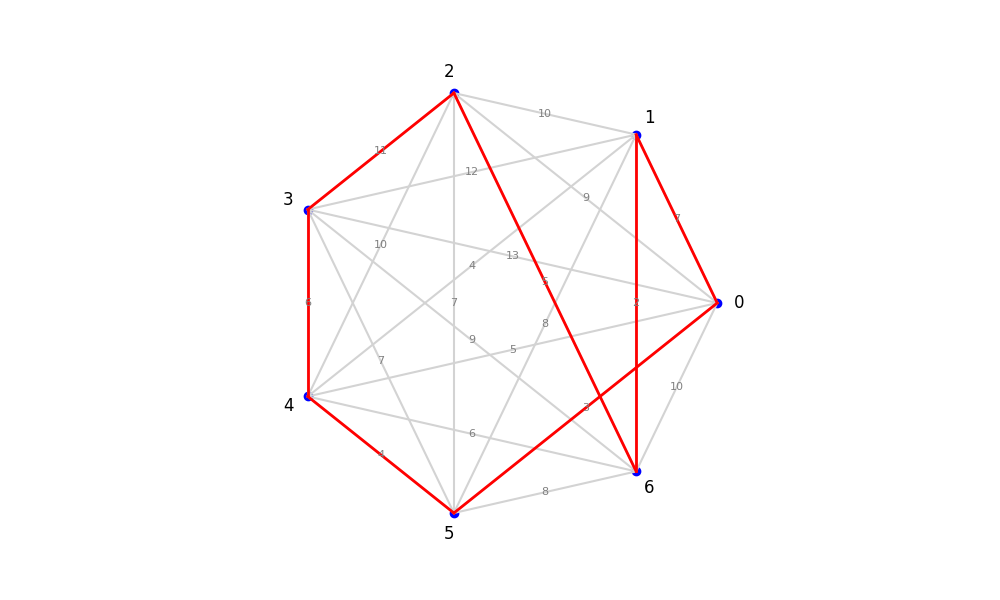
\includegraphics[width=0.9\textwidth]{Figures/QuickInsertion}
\end{center}

	
	
	
	
	
	\begin{theorem}
		The performance guarantee of Quick Insertion Method is $2$.
	\end{theorem}
	

	
	\subsection{Christofides Algorithm} 
	
	\begin{algorithm}
		\caption{Christofides' Algorithm (1976)}
		\begin{algorithmic}[1] % The number [1] indicates that lines are numbered
			\State Compute a minimum spanning tree $T$ in $G$.
			\State Let $U$ denote the set of all vertices with odd degree in $T$. Compute a minimum weighted perfect matching $M$ in $G[U]$, the graph induced by $U$ in $G$.
			\State Compute an Eulerian tour $W$ on $H = T + M$. Convert $W$ into a Hamiltonian cycle $C$ by making a short cut. Return $C$.
		\end{algorithmic}
	\end{algorithm}
	We implement our code here, which demonstrates the algorithm running on a complete graph with 5 vertices: 
	
	

	
	

		
		\begin{multicols}{3} % Adjust the number '2' to '3' or more depending on your preference and the size of the images
			
			\begin{figure}[H]
				\centering
				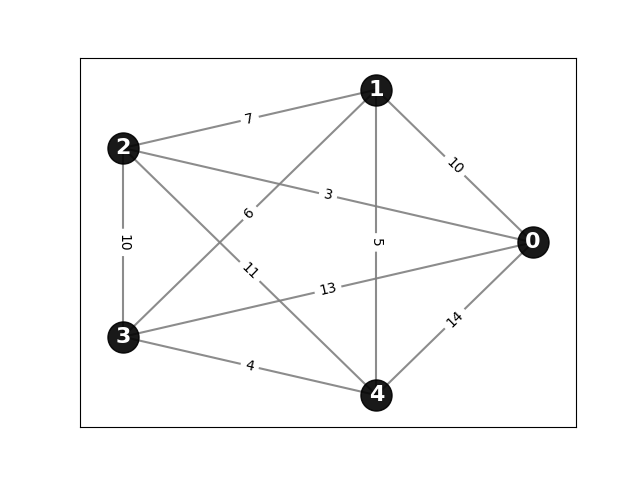
\includegraphics[width=\linewidth]{Figures/Christo_0.png}
				\caption{Initial Placement}
			\end{figure}
			
			\begin{figure}[H]
				\centering
				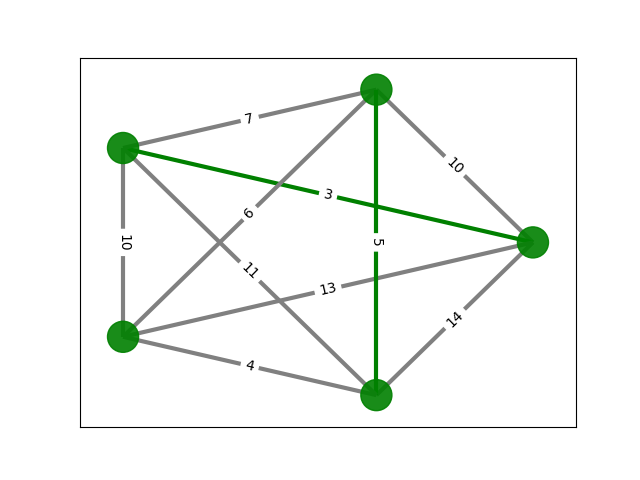
\includegraphics[width=\linewidth]{Figures/Christo_1.png}
				\caption{Finding MST}
			\end{figure}
			
			\begin{figure}[H]
				\centering
				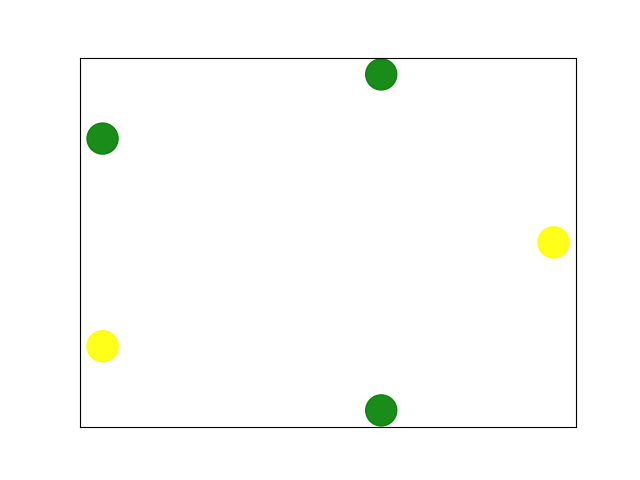
\includegraphics[width=\linewidth]{Figures/Christo_2.png}
				\caption{Vertices of odd degree in MST}
			\end{figure}
			
			\begin{figure}[H]
				\centering
				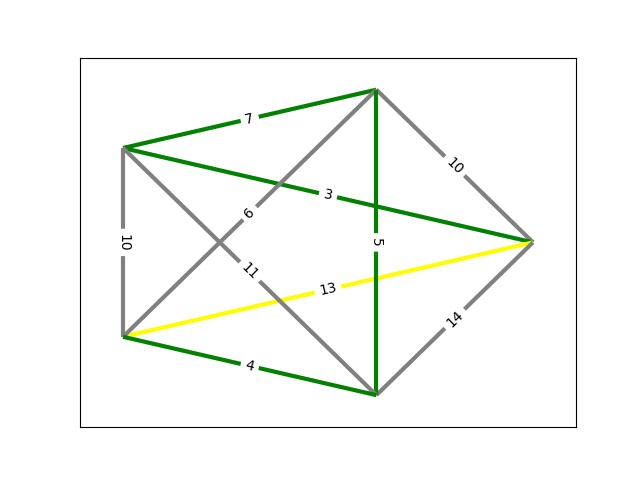
\includegraphics[width=\linewidth]{Figures/Christo_3.png}
				\caption{Minimum weight matching in induced subgraph}
			\end{figure}
			
			\begin{figure}[H]
				\centering
				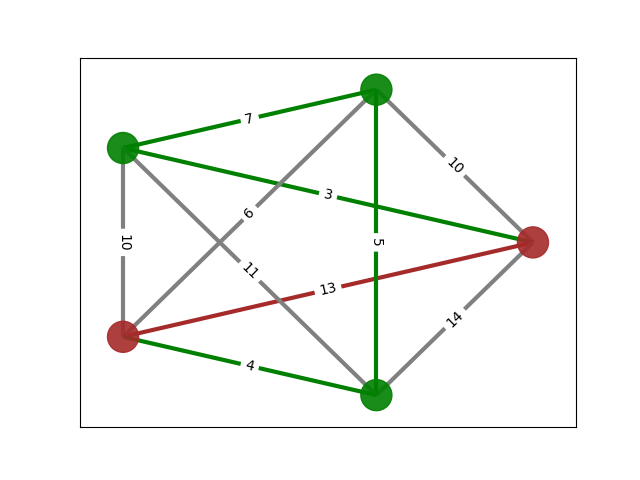
\includegraphics[width=\linewidth]{Figures/Christo_4.png}
				\caption{Combine the matching and MST}
			\end{figure}
			
			\begin{figure}[H]
				\centering
				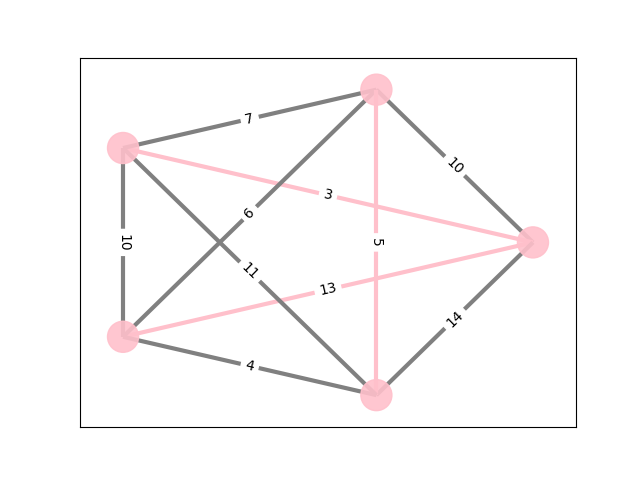
\includegraphics[width=\linewidth]{Figures/Christo_5.png}
				\caption{Eulerian circuit}
			\end{figure}
			
			
			
	
		\end{multicols}
\begin{figure}[H]
	\centering
	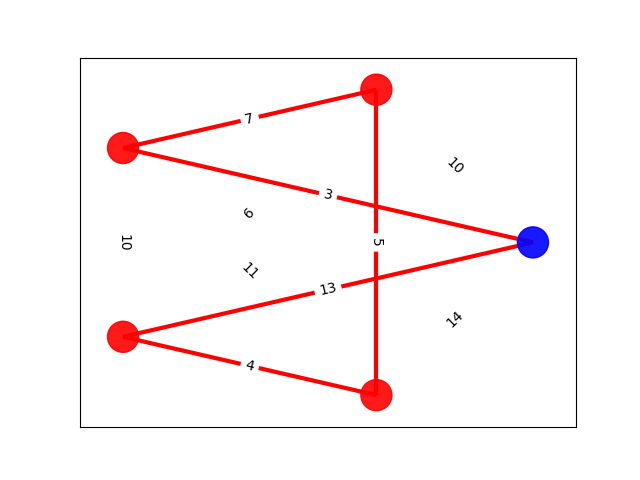
\includegraphics[width=0.6\linewidth]{Figures/Christo_6.png}
	\caption{Final Hamiltonian cycle}
\end{figure}
	
\begin{theorem}\label{thm:christofides}
	The performance guarantee of Christofides algorithm is $1.5.$
\end{theorem}

\begin{proof}[Proof sketch]
	The proof relies on three key inequalities. First, by the triangle inequality and the construction of $C$, we have $c(C) \leq c(T) + c(M)$. Second, since any Hamiltonian cycle minus one edge forms a spanning tree, the optimal tour satisfies $c(C^\star) \geq c(T)$. Third, by constructing two specific matchings from the optimal tour and applying the triangle inequality, we show that $c(M) \leq \frac{c(C^\star)}{2}$. Combining these three inequalities yields $c(C) \leq 1.5c(C^\star)$.
	
	The complete proof is provided in Appendix~\ref{app:christofides}.
\end{proof}


	Additionally, an animated demonstration of the Christofides algorithm was developed using the Manim animation engine, available for viewing at: \url{https://liu-zhonglin.github.io/Christofides-vs-RL-for-TSP/Project%20Report/Christofides.mp4}
	
	
\section{Reinforcement Learning for the TSP}

\subsection{Model Architecture: Pointer Network with Attention}
The core of the learning-based approach is a sequence-to-sequence model known as a Pointer Network \cite{vinyals2015pointer}. This architecture is particularly well-suited for combinatorial optimization problems where the output is a permutation of the input, a task for which standard sequence-to-sequence models that output to a fixed-size dictionary are ill-suited. The model leverages an encoder-decoder structure augmented with an attention mechanism, a paradigm that has proven highly effective in fields such as natural language translation \cite{bahdanau2014neural} and has been further revolutionized by the introduction of the Transformer architecture \cite{vaswani2017attention}.

The model's process begins with an encoder, implemented as a Long Short-Term Memory (LSTM) network \cite{hochreiter1997long}. The encoder's role is to create a rich, contextual representation of the entire input TSP problem. Given an input sequence of $n$ city coordinates $X = (x_1, x_2, \dots, x_n)$, where each $x_i \in \mathbb{R}^2$, the encoder processes this sequence to produce a set of hidden state embeddings $E = (e_1, e_2, \dots, e_n)$. Each embedding $e_j \in \mathbb{R}^h$ (for a hidden dimension $h$) contains information about a specific city in the context of all other cities. The final hidden and cell states of the encoder, $(h_n, c_n)$, serve as a summary of the entire problem instance and are used to initialize the decoder.

The decoder, also an LSTM, is tasked with autoregressively constructing the output tour $\pi = (\pi_1, \pi_2, \dots, \pi_n)$ by "pointing" to one of the input cities at each decoding step. This pointing mechanism is achieved through a content-based attention mechanism \cite{luong2015effective}. While the Transformer architecture has demonstrated that attention mechanisms alone can be sufficient for sequence transduction tasks \cite{vaswani2017attention}, our approach combines attention with recurrent components to maintain the sequential nature required for TSP tour construction. At each decoding step $i$, the decoder's current hidden state, $d_i$, is used as a "query" to the attention mechanism. This mechanism computes an alignment score, $u_{ij}$, for each of the encoder's hidden states $e_j$, measuring how relevant input city $j$ is to the current state of the tour construction. We use additive attention \cite{bahdanau2014neural}, formulated as:
$$ u_{ij} = v^T \tanh(W_1 e_j + W_2 d_i) $$
where $W_1$, $W_2$, and $v$ are learnable weight parameters.

To ensure a valid TSP tour is generated, a mask is applied to the scores at each step, setting the score of any previously visited city to $-\infty$. This prevents the model from selecting the same city twice. The masked scores are then converted into a probability distribution over the input cities using the softmax function, which represents the model's policy:
$$ p(\pi_i = j | \pi_{1..i-1}, X) = \frac{\exp(u_{ij})}{\sum_{k=1}^{n} \exp(u_{ik})} $$
The city with the highest probability is then selected as the next city in the tour, $\pi_i$, and its coordinates become the input for the subsequent decoder step. This process repeats for $n$ steps, generating a full permutation of the input cities, which constitutes the final TSP tour.
	
	\begin{figure}[h!]
		\centering
		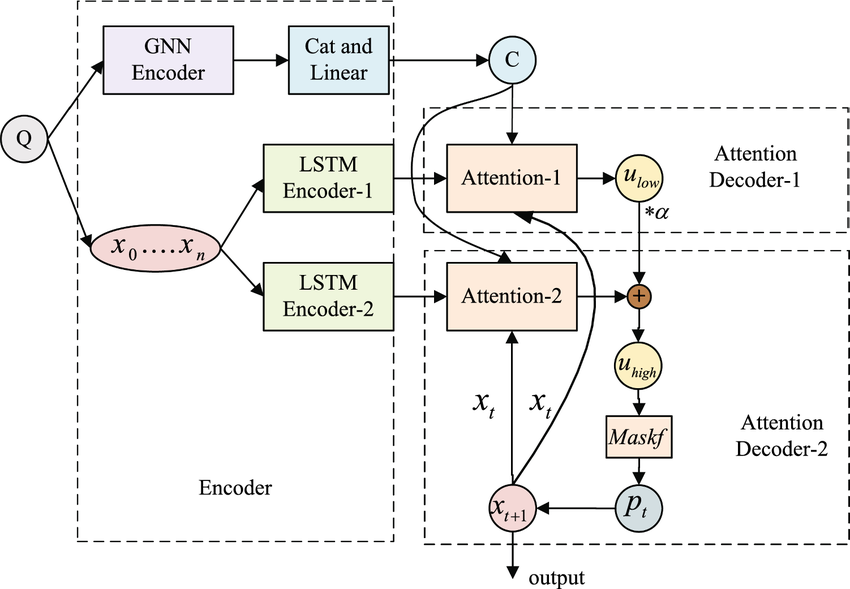
\includegraphics[width=0.7\textwidth]{Figures/pointer_network_diagram.png} % You would need to create this diagram
		\caption{A simplified diagram of the Pointer Network architecture, showing the encoder processing all inputs and the decoder pointing to one input at each step via the attention mechanism.}
		\label{fig:pointer_network}
	\end{figure}
	
\subsection{Training Paradigms}
To thoroughly investigate the impact of different learning strategies, three distinct RL agents were trained on 30-city problems, each for 5000 epochs. The best-performing model weights from each training run were preserved for the final evaluation.

\subsubsection{Pure RL with REINFORCE}
The first model served as a baseline to evaluate the performance of the Pointer Network architecture in isolation. It was trained using the REINFORCE policy gradient algorithm \cite{williams1992simple}. For each training step, a batch of TSP instances was generated with city coordinates in a random, unordered sequence. The model's objective is to minimize the expected tour length. The loss function for a single instance is defined as:
$$ \mathcal{L}(\theta) = \mathbb{E}_{\pi_\theta} [L(\pi)] $$
where $L(\pi)$ is the length of the tour $\pi$ generated by the policy $\pi_\theta$ with parameters $\theta$. The gradient is estimated using the REINFORCE rule:
$$ \nabla_\theta \mathcal{L}(\theta) \approx L(\pi) \nabla_\theta \log p(\pi | X; \theta) $$
Here, $L(\pi)$ serves as the reward signal. By performing gradient descent on this objective, the model updates its weights to increase the probability of generating shorter tours.

\subsubsection{Hybrid RL with REINFORCE}
The second agent was designed to test the hypothesis that providing structural information from a classical algorithm could improve learning. The training process was identical to the pure RL model, using the same REINFORCE algorithm. However, the input sequence of city coordinates, $X$, was not random. Instead, for each problem instance, the Christofides algorithm was first run to generate an Eulerian tour. This tour was then converted into a valid Hamiltonian cycle via a deterministic shortcutting heuristic. The resulting high-quality tour provided the ordered sequence of cities that was fed into the Pointer Network. The agent's task was thus transformed from solving the problem from scratch to learning how to improve upon an already excellent solution.

\subsubsection{Hybrid RL with Actor-Critic}
The third and most advanced agent builds upon the hybrid approach by using a more stable training algorithm known as an Actor-Critic method \cite{sutton1998reinforcement}. This paradigm introduces a second neural network, the Critic ($V_\phi$), whose purpose is to estimate the value (expected tour length) of a given state, thereby providing a more refined learning signal.

The training process begins with the Actor ($\pi_\theta$, our Pointer Network) taking the Christofides-ordered city sequence and producing a tour $\pi$ along with its log-probability, $\log p(\pi | X; \theta)$. The final hidden state from the Actor's decoder, $s$, is then passed to the Critic, which outputs a value estimate, $V_\phi(s)$. This value represents the Critic's prediction of the tour length given the state. The actual tour length, $L(\pi)$, is then calculated to serve as the ground-truth reward.

A key concept in this method is the Advantage, $A$, which measures how much better or worse the Actor's tour was compared to the Critic's expectation. It is defined as $A = L(\pi) - V_\phi(s)$. To prevent the Actor's loss from influencing the Critic's training, the value term $V_\phi(s)$ is detached from the computation graph during this step. The model is then updated by optimizing a combined loss function. The Actor Loss is designed to reinforce actions that led to a positive advantage, effectively encouraging policies that outperform the Critic's baseline. Its gradient is given by:
$$ \nabla_\theta \mathcal{L}_{actor}(\theta) = -A \cdot \nabla_\theta \log p(\pi | X; \theta) $$
Simultaneously, the Critic Loss is updated via a standard Mean Squared Error loss, which trains the Critic to make its value predictions, $V_\phi(s)$, more accurate with respect to the true tour length, $L(\pi)$:
$$ \mathcal{L}_{critic}(\phi) = (L(\pi) - V_\phi(s))^2 $$
This method generally leads to more stable training than REINFORCE because the advantage signal is less noisy than using the raw reward alone.


\section{Results and Discussions}
To provide a definitive and statistically sound comparison, a final robust evaluation was conducted. Each of the five developed methods was tested on 1000 unique, randomly generated TSP instances for both 30-city and 100-city problem sizes. The average tour length and average computation time were recorded to compare performance and scalability.


The TSP instances were generated by uniformly sampling city coordinates in a $[0, 1] \times [0, 1]$ unit square. This ensures that the edge weights, calculated as the Euclidean distance between cities, satisfy the triangle inequality, making it a valid Metric TSP for which the classical heuristics are appropriate.

The key hyperparameters for all reinforcement learning models were kept consistent to ensure a fair comparison. A hidden dimension of 128 was used for the LSTM cells in the Pointer Network, a standard size that provides sufficient capacity for learning complex patterns. A batch size of 128 was used during training to offer a good balance between stable gradient estimates and memory usage. For the Adam optimizer, a learning rate of $1 \times 10^{-4}$ was chosen, as a small rate is standard for policy gradient methods to prevent destructively large updates and promote stable convergence. All RL models were trained for 5000 epochs to provide ample opportunity to converge, and the model weights that achieved the best average tour length during this period were saved and used for the final evaluation. The final evaluation itself was performed over 1000 trials for each problem size to ensure the reported average performance is statistically robust and not the result of outlier instances.

\subsection{Experimental Results}
The aggregated results from the 1000-trial evaluations for both problem scales are presented below in Table \ref{tab:combined_results}. Figure \ref{fig:scaling_comparison} provides a visual summary of the tour length results, illustrating how each algorithm's performance scales with problem size.

\begin{table}[h!]
	\centering
	\captionsetup{justification=centering}
	\caption{Final Results (1000 Trials)}
	\label{tab:combined_results}
	\resizebox{\textwidth}{!}{%
		\begin{tabular}{l|l|ccccc}
			\toprule
			\multicolumn{2}{c|}{\textbf{Metric}} & \textbf{Christofides} & \textbf{Nearest Insertion} & \textbf{Pure RL} & \textbf{Hybrid (REINFORCE)} & \textbf{Hybrid (Actor-Critic)} \\
			\midrule
			\multirow{2}{*}{\textbf{Avg. Tour Length}} & 30 Cities & 5.3300 & 5.2107 & 11.9242 & 10.5369 & 10.3699 \\
			& 100 Cities & 9.3701 & 9.3125 & 32.4112 & 26.9063 & 9.3705 \\
			\midrule
			\multirow{2}{*}{\textbf{Avg. Comp. Time (s)}} & 30 Cities & 0.0005 & 0.0005 & 0.0222 & 0.0218 & 0.0216 \\
			& 100 Cities & 0.0013 & 0.0137 & 0.0740 & 0.0733 & 0.0741 \\
			\bottomrule
	\end{tabular}}
\end{table}

\begin{figure}[h!]
	\centering
	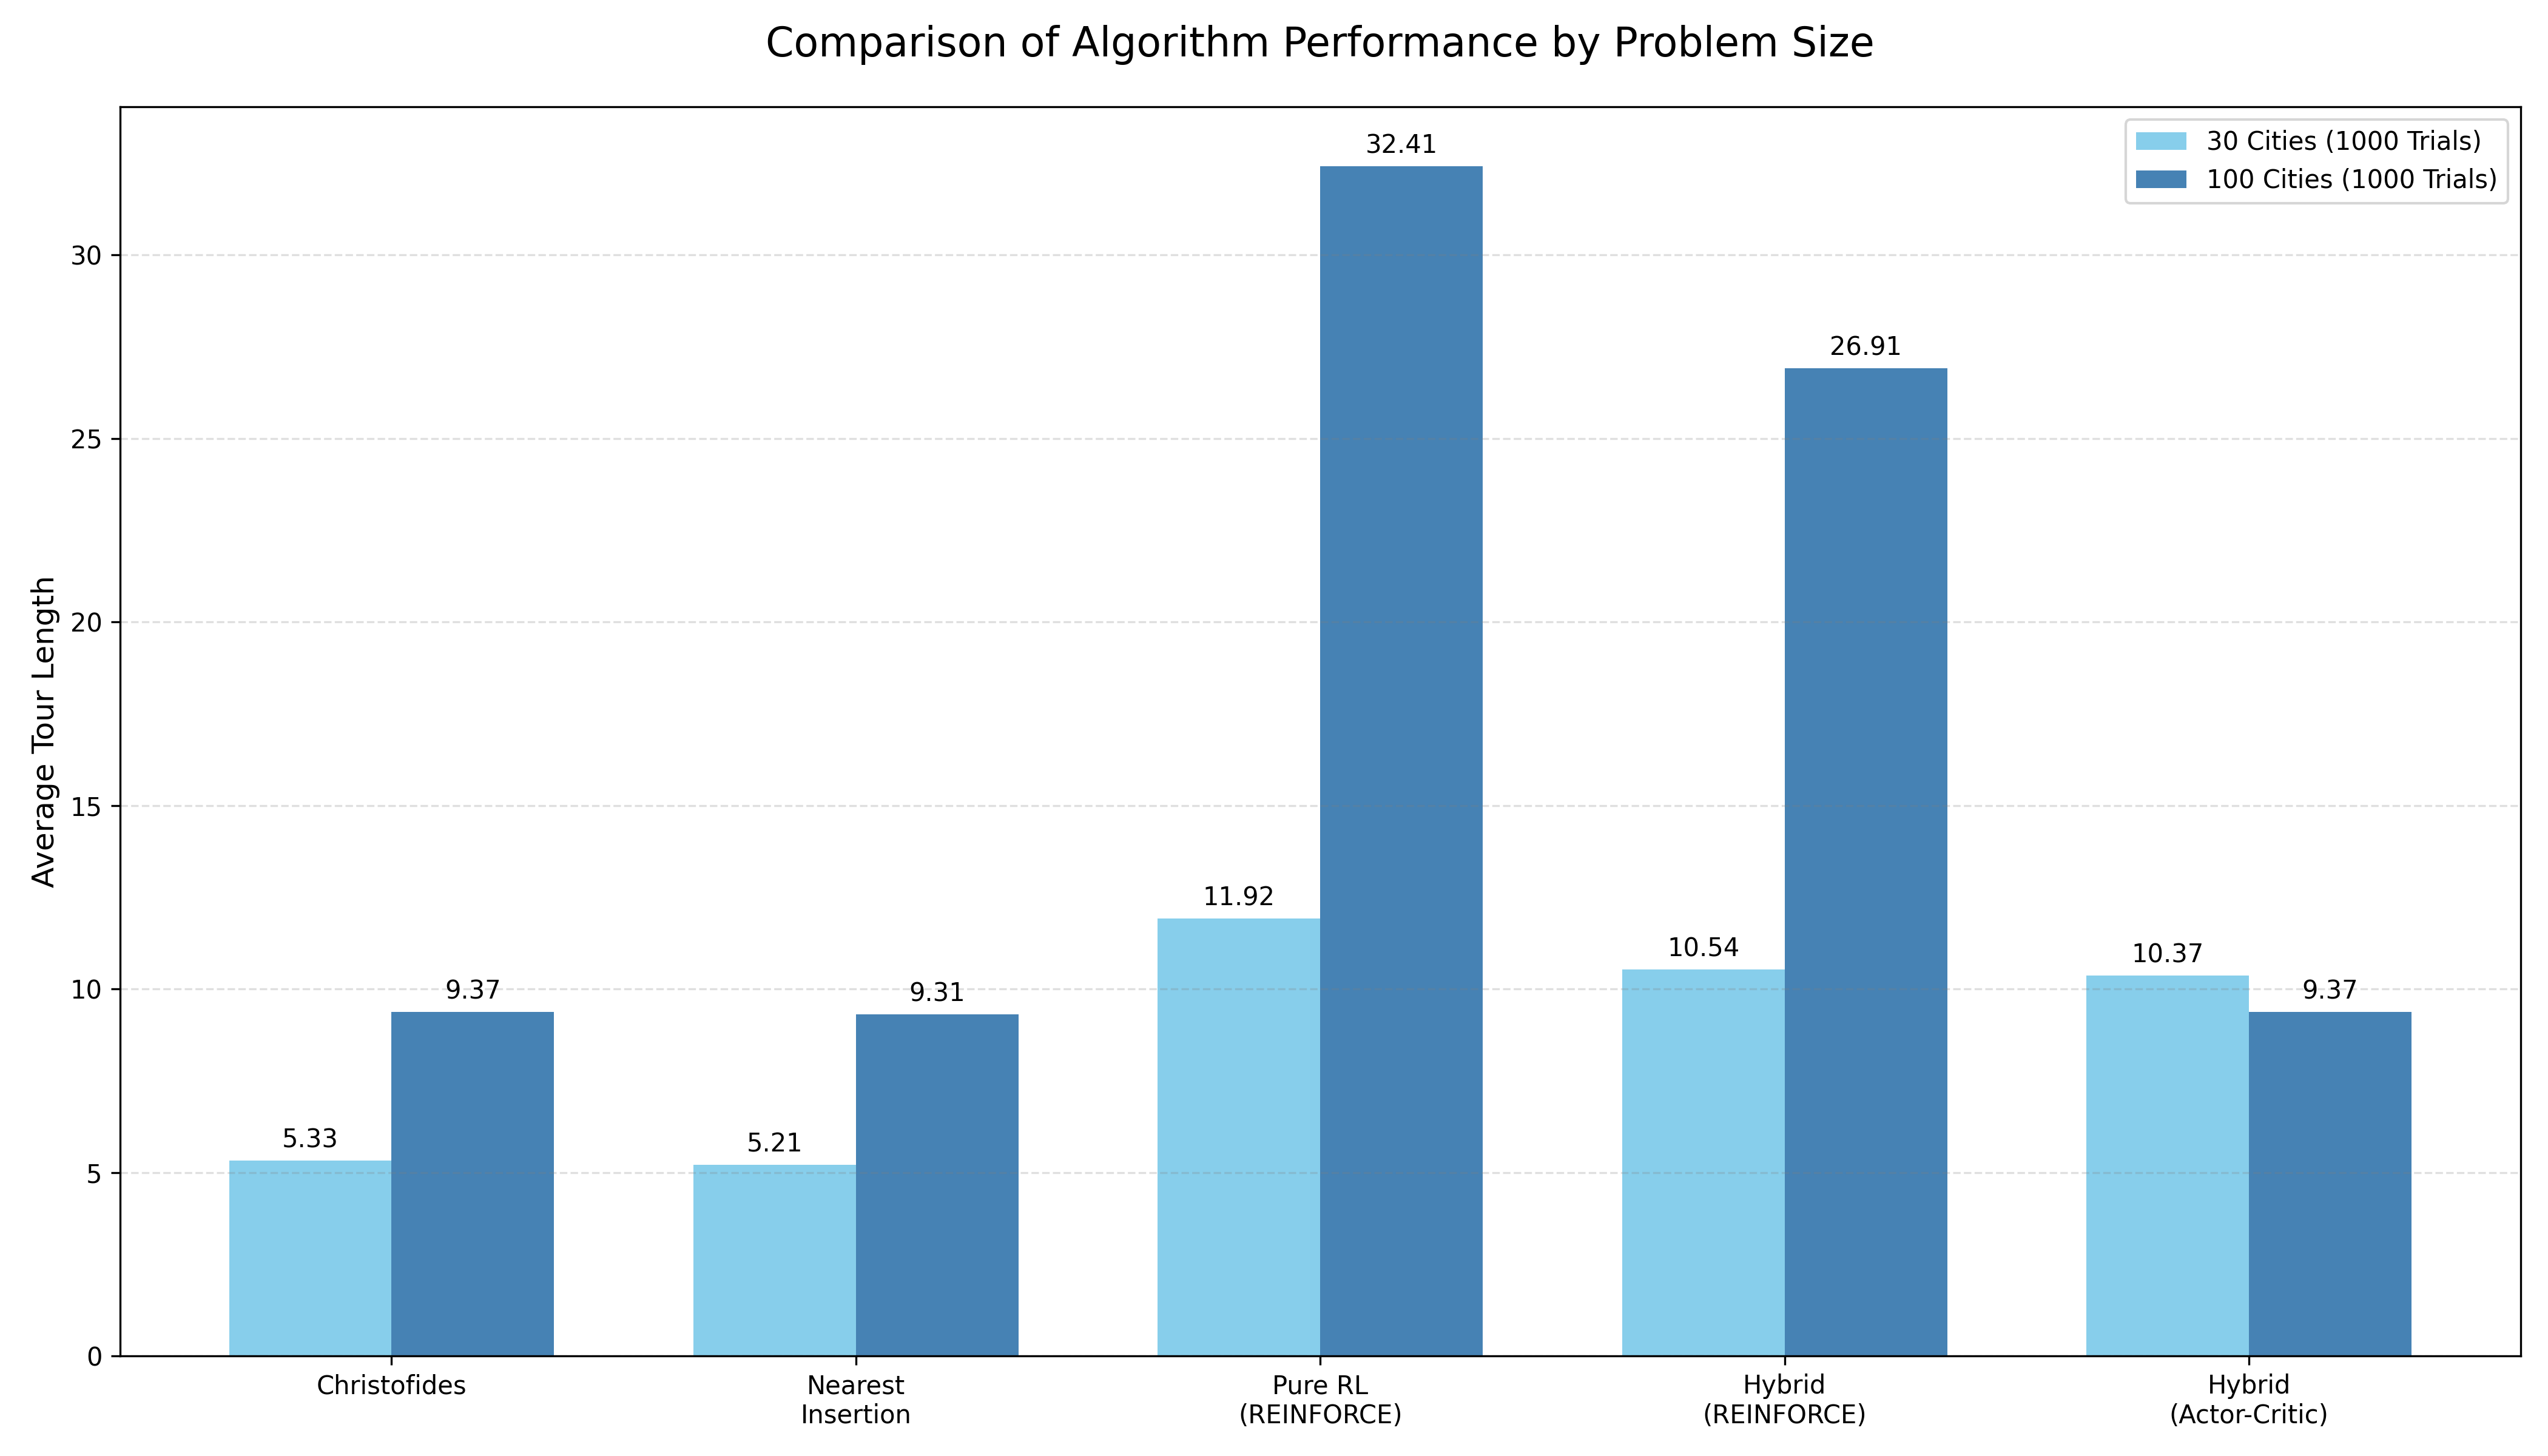
\includegraphics[width=\textwidth]{Figures/final_scaling_comparison.png}
	\caption{A grouped bar chart comparing the average tour length of each algorithm across both 30-city and 100-city problem sizes.}
	\label{fig:scaling_comparison}
\end{figure}

\subsection{Discussion}
The comprehensive evaluation reveals several key insights into the performance and characteristics of these different approaches.

Across both 30-city and 100-city scales, the classical heuristics proved vastly superior to the reinforcement learning models in both solution quality and computational speed. Interestingly, the simpler Nearest Insertion heuristic consistently found slightly better average solutions than the Christofides algorithm, which has a stronger theoretical worst-case guarantee. This highlights a common phenomenon in practice where simpler, greedy methods can outperform more complex algorithms on average problem instances. Their sub-second computation times confirm their suitability for real-world applications where speed is critical.

A crucial finding is the dramatic performance gap between the pure RL model and the hybrid models. At both scales, the pure RL agent, which learned from randomly ordered inputs, produced significantly longer tours than the hybrid agents, which were given a Christofides-ordered sequence. This demonstrates that providing the learning agent with a high-quality structural "hint" from a classical algorithm is a highly effective strategy for improving performance and guiding the learning process.

The most striking result is the performance of the Hybrid (Actor-Critic) model on the 100-city problem. While the simpler Hybrid (REINFORCE) model's performance degraded significantly at the larger scale, the Actor-Critic model's performance was outstanding, achieving an average tour length statistically identical to that of the powerful Christofides and Nearest Insertion heuristics. This shows that for complex, large-scale problems, a stable learning algorithm like Actor-Critic is not just a minor improvement; it is the critical factor that enables the RL agent to effectively learn a competitive policy.

This study confirms that while classical heuristics remain the benchmark for the standard Euclidean TSP, the potential of reinforcement learning is unlocked through intelligent integration with classical methods. The success of the Actor-Critic hybrid model demonstrates that by combining the structural knowledge of classical algorithms with the stable learning signal of advanced RL techniques, it is possible to train agents that can achieve performance competitive with strong, specialized heuristics.


\section{Conclusion}
This directed study successfully implemented and rigorously evaluated a range of solution methods for the Traveling Salesman Problem, from established classical heuristics to modern deep reinforcement learning agents. The comprehensive, multi-trial evaluation across different problem scales provided a clear and definitive performance hierarchy.

The results reaffirm the efficacy and efficiency of classical approximation algorithms like Nearest Insertion and Christofides, which consistently produced the highest-quality solutions in a fraction of the time required by the learning-based models. However, the study's most significant contribution lies in its investigation of hybrid reinforcement learning. The experiments conclusively demonstrate that while a pure RL agent struggles to scale effectively, its performance can be dramatically improved by integrating domain knowledge from classical algorithms. Furthermore, the outstanding performance of the Actor-Critic hybrid model on the 100-city problem underscores the critical importance of using advanced, stable training algorithms to tackle complex optimization tasks.

Ultimately, this research points to a promising direction for applying machine learning to combinatorial optimization—not as a replacement for classical methods, but as a means of building sophisticated hybrid systems. By combining the structural insights of classical theory with the flexible learning capabilities of modern neural networks, we can develop agents whose performance rivals that of strong, specialized heuristics.
	
	\section*{Code Availability}
	The complete Python source code for all classical algorithms, reinforcement learning models, training scripts, and evaluation protocols developed in this study is publicly available on GitHub at the following repository: \url{https://github.com/Liu-Zhonglin/Christofides-vs-RL-for-TSP}
	
	
	\section*{Acknowledgment}
	
	I would like to extend my sincere gratitude to Prof. Zang Wenan, a leading expert in graph theory and discrete optimization, for his invaluable guidance and support throughout my capstone course, MATH3999: Directed Studies in Mathematics. His insightful advice has been instrumental in shaping my understanding of graph theory and discrete optimization, as well as in directing my independent research. Under his recommendation, I concurrently enrolled in MATH3943: Network Models in Operations Research during the academic year 2024. This course provided an excellent introduction to graph theory and a solid foundation for exploring the theoretical aspects of algorithms, complementing the research I undertook in MATH3999.
	
	I would also like to express my heartfelt appreciation to the Mathematics Department of HKU, which fosters creative thinking and provides a strong foundation for both teaching and research. I was honored to attend the Frontiers of Mathematics Lecture, themed “The Salesman and the Postman: Frontiers and Gateways in Combinatorial Optimization”, organized by the department. This lecture offered valuable insights into how the Chinese Postman Problem can inspire innovative approaches to tackling the Traveling Salesman Problem (TSP), further enriching my understanding of combinatorial optimization.


	
	

% --- USE THIS VERSION FOR A TWO-COLUMN DOCUMENT ---
\begin{figure*}[h!] % Note the asterisk here!
	\centering
	
	\begin{subfigure}{0.48\textwidth} % Note textwidth instead of linewidth
		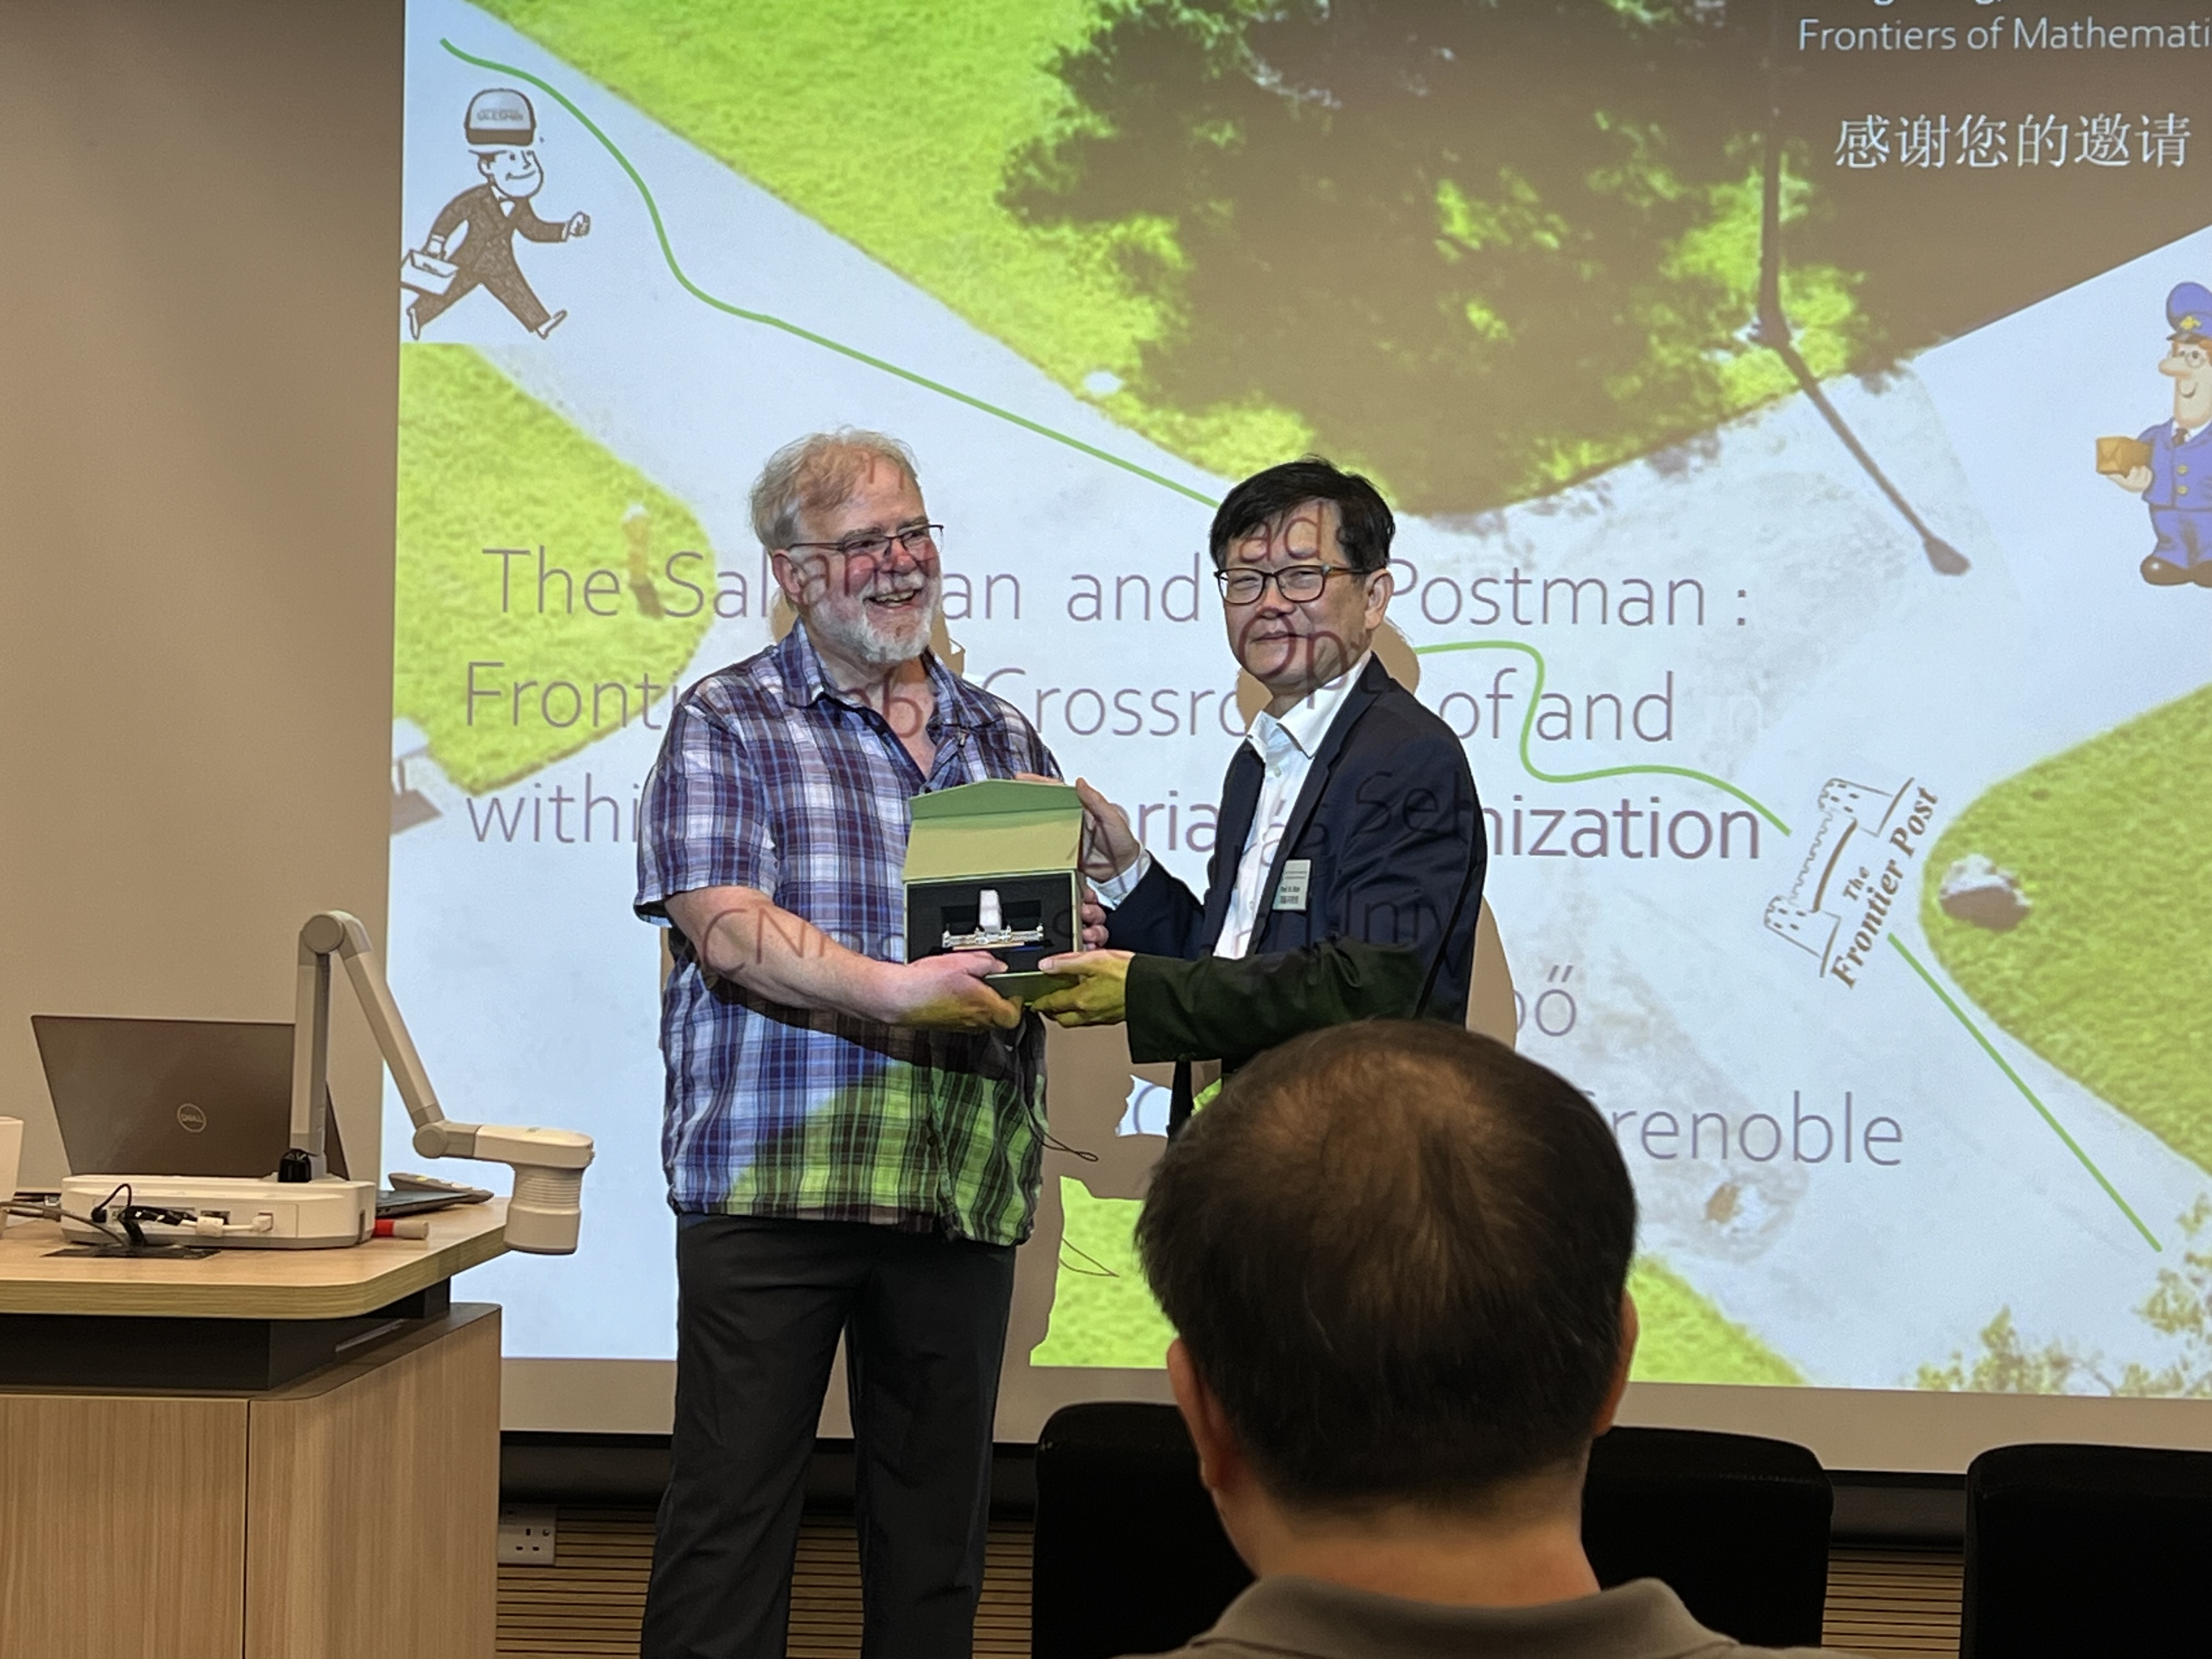
\includegraphics[width=\linewidth]{Figures/Thetalk1}
		\caption{Frontiers of Mathematics Lecture (1)}
		\label{fig:talk1}
	\end{subfigure}
	\hfill
	\begin{subfigure}{0.48\textwidth} % Note textwidth instead of linewidth
		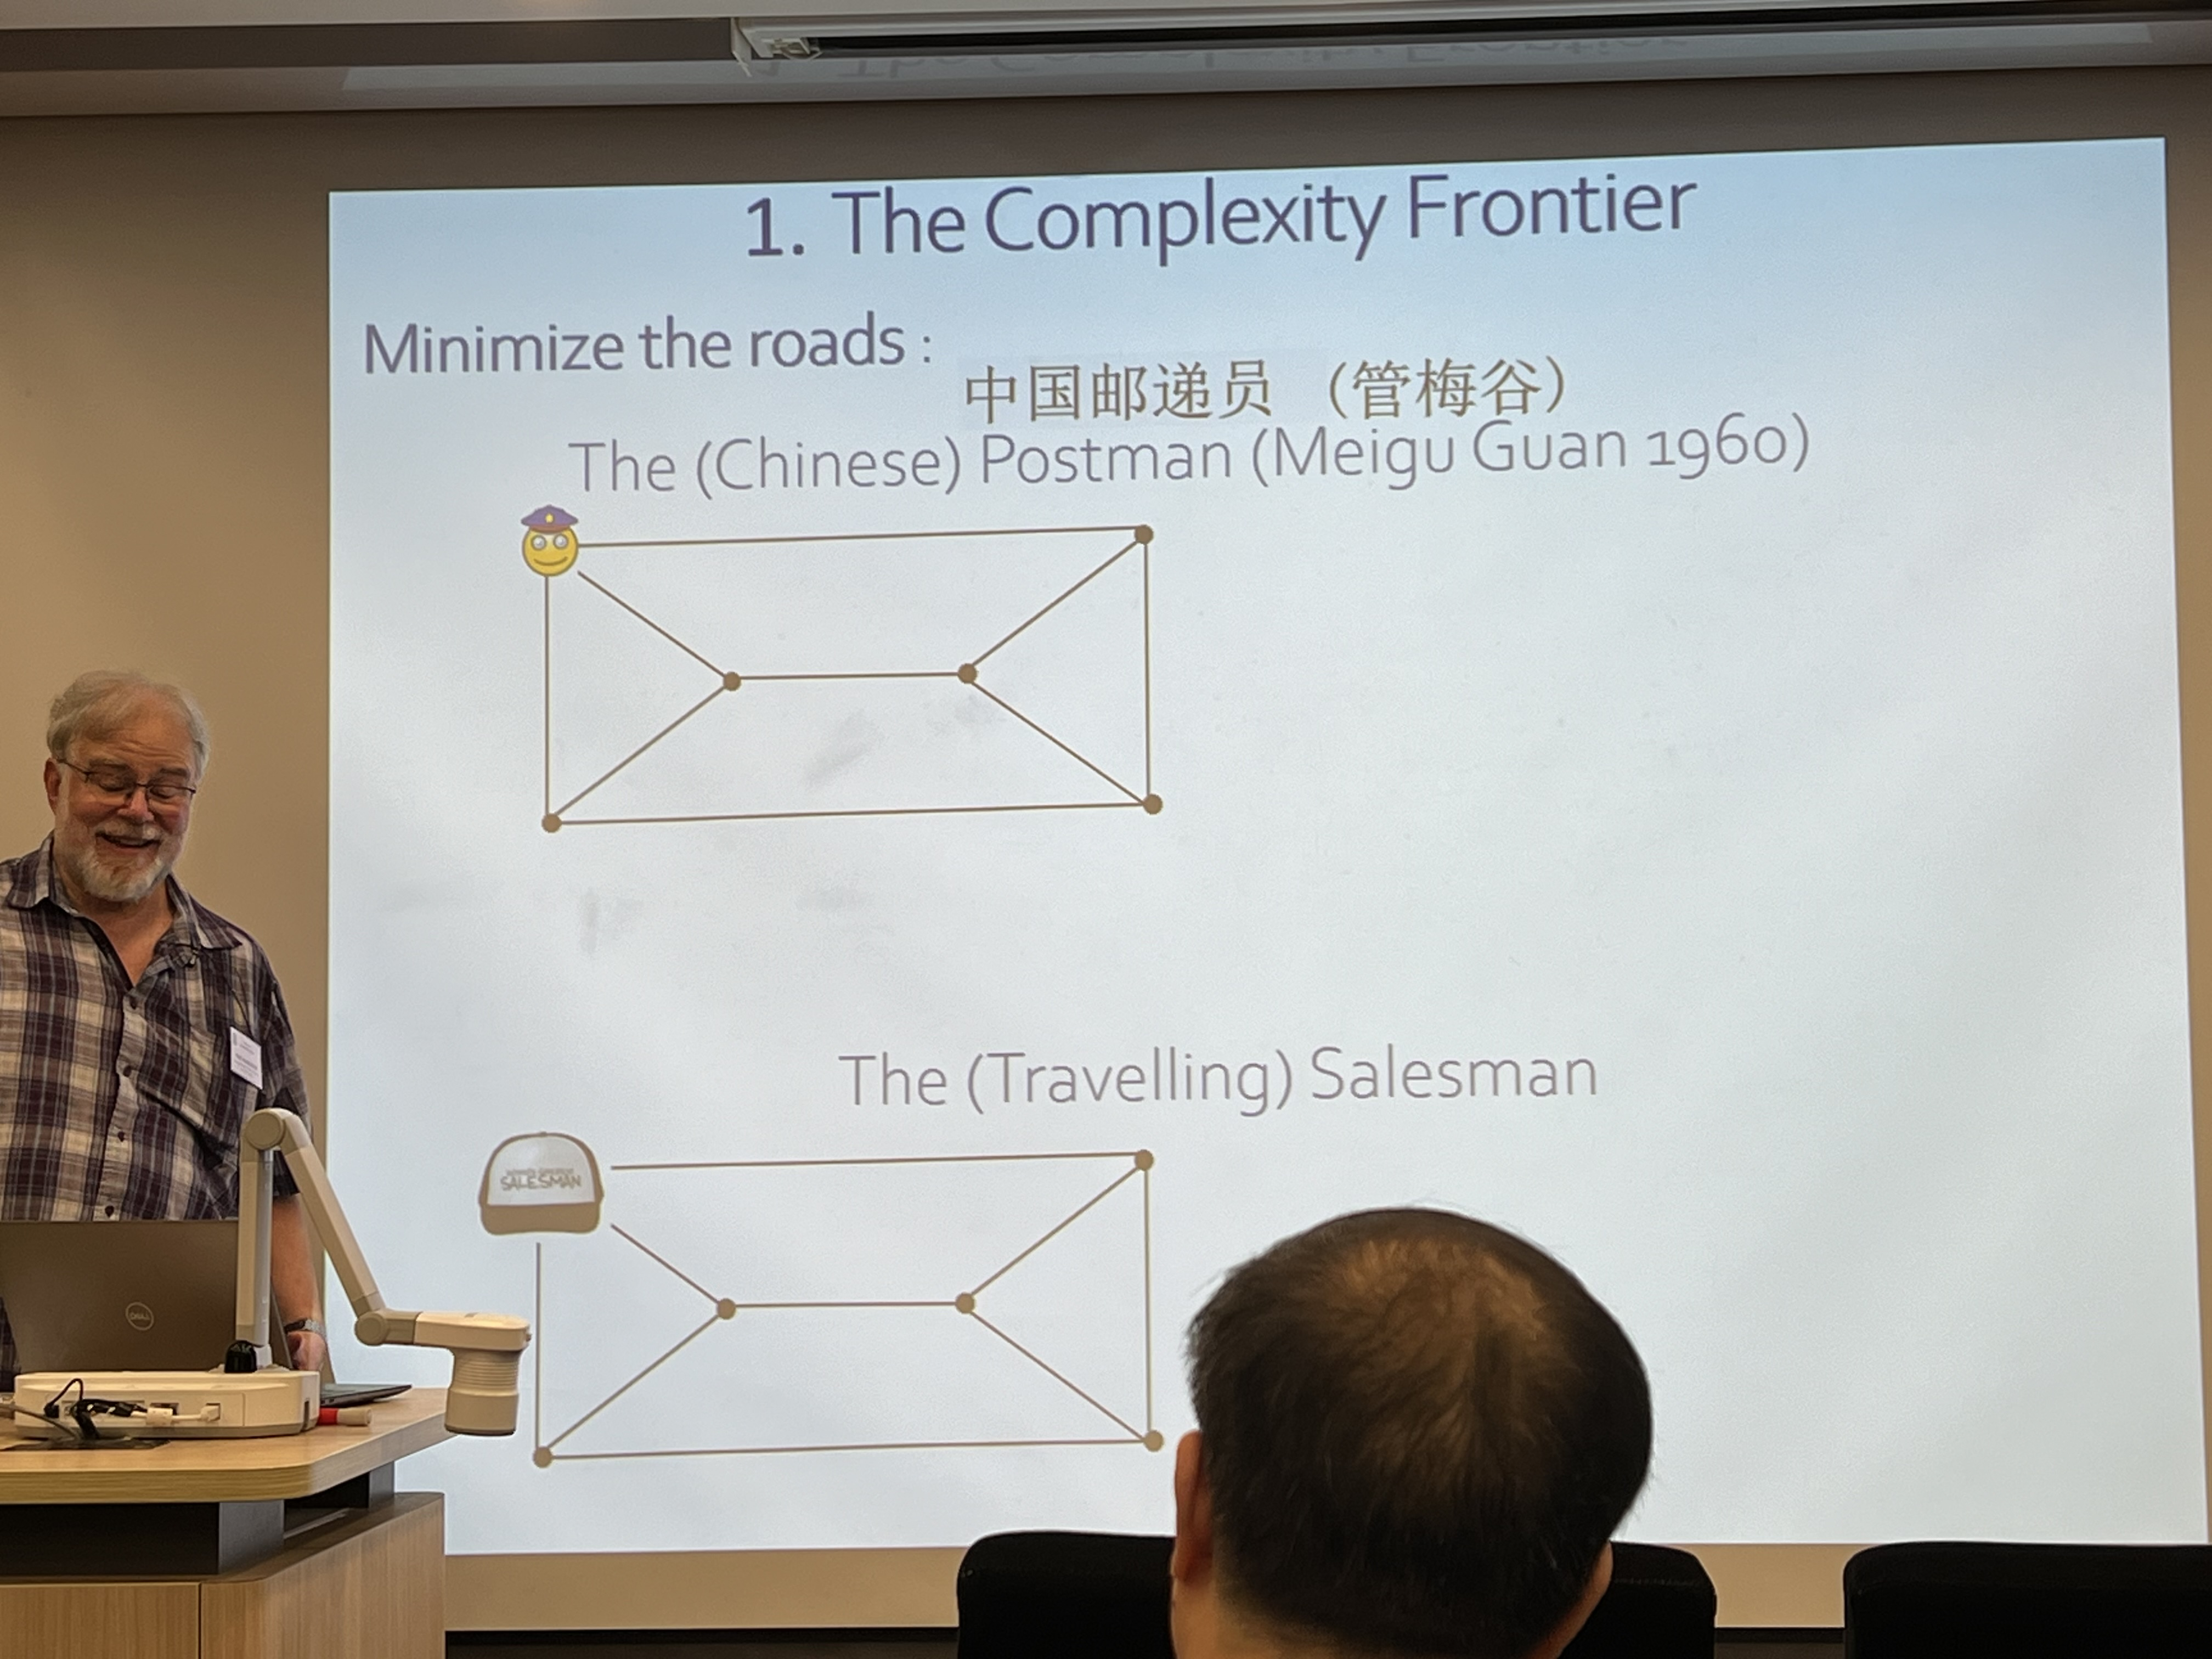
\includegraphics[width=\linewidth]{Figures/Thetalk2}
		\caption{Frontiers of Mathematics Lecture (2)}
		\label{fig:talk2}
	\end{subfigure}
	
	\caption{Photos from the Frontiers of Mathematics Lecture.}
	\label{fig:talk_photos}
\end{figure*}
	

	
	In conclusion, I am deeply grateful for the opportunities and support I have received during this capstone course and my studies at HKU. These experiences have significantly enhanced my knowledge and skills in mathematics, particularly in the field of optimization. I look forward to applying what I have learned to future challenges and contributing to advancements in this exciting area of research
	

\bibliographystyle{plain}
\bibliography{references} 
	
	
	
\appendix

\section{Proofs}

\begin{proof}[Proof of Theorem~\ref{thm:christofides}]\label{app:christofides}
	Since the weight function satisfies the triangle inequality, according to the construction of $C$, we have 
	\begin{equation}
		c(C) \leq c(W) = c(T) + c(M),
		\label{eq:christofides1}
	\end{equation}
	where $c(A)$ stands for the total weight of $A$ with respect to $c$.
	
	Now let $C^\star$ be a minimum Hamiltonian cycle of $G$. Then 
	\begin{equation}
		c(C^\star)\geq c(T).
		\label{eq:christofides2}
	\end{equation}
	Indeed, for any edge $e$ on $C^\star$, $C^\star-e$ is a spanning tree of $G$. So $c(C^\star-e)\geq c(T)$ and thus \eqref{eq:christofides2} follows.
	
	Let $\{i_1,i_2,\dots,i_{2m}\}$ be the vertices in $U$ in step $2$, in the order they appear in $C^\star.$ Consider two matchings of $U$:
	\begin{align*}
		&M_1=\{i_1i_2,i_3i_4,\dots,i_{2m-1}i_{2m}\},\\
		&M_2=\{i_2i_3,i_4i_5,\dots,i_{2m}i_1\}.
	\end{align*}
	By the triangle inequality, $c(C^\star)\geq c(M_1)+c(M_2).$ Since $M$ is a minimum perfect matching of $G[U]$, $c(M_1)\geq c(M)$ and $c(M_2)\geq c(M).$ Thus $c(C^\star)\geq 2c(M)$ or 
	\begin{equation}
		c(M)\leq \frac{c(C^\star)}{2}.
		\label{eq:christofides3}
	\end{equation}
	Combining \eqref{eq:christofides1}, \eqref{eq:christofides2} and \eqref{eq:christofides3}, we have 
	$$c(C)\leq c(T) + c(M) \leq c(C^\star) + \frac{c(C^\star)}{2} = 1.5c(C^\star).$$
\end{proof}



\end{document}